%保存为UTF-8编码格式
%用xelatex编译
 
\documentclass[UTF8,a4paper,12pt]{ctexart}
\usepackage[left=2.50cm, right=2.50cm, top=2.50cm, bottom=2.50cm]{geometry} %页边距
\CTEXsetup[format={\Large\bfseries}]{section} %设置章标题字号为Large,居左
%\CTEXsetup[number={\chinese{section}}]{section}
%\CTEXsetup[name={(,)}]{subsection}
%\CTEXsetup[number={\chinese{subsection}}]{subsection}
%\CTEXsetup[name={(,)}]{subsubsection}
%\CTEXsetup[number=\arabic{subsubsection}]{subsubsection}  %以上四行为各级标题样式设置,可根据需要做修改
 
%\linespread{1.5} %设置全文行间距
 
 
%\usepackage[english]{babel}
%\usepackage{float}     %放弃美学排版图表
\usepackage{fontspec}   %修改字体
\usepackage{amsmath, amsfonts, amssymb} % 数学公式相关宏包
\usepackage{color}      % color content
\usepackage{graphicx}   % 导入图片
\usepackage{subfigure}  % 并排子图
\usepackage{url}        % 超链接
\usepackage{bm}         % 加粗部分公式,比如\bm{aaa}aaa
\usepackage{multirow}
\usepackage{booktabs}
\usepackage{epstopdf}
\usepackage{epsfig}
\usepackage{longtable}  %长表格
\usepackage{supertabular}%跨页表格
\usepackage{algorithm}
\usepackage{algorithmic}
\usepackage{changepage}
 
 
 
%%%%%%%%%%%%%%%%%%%%%%%
% -- text font --
% compile using Xelatex
%%%%%%%%%%%%%%%%%%%%%%%
% -- 中文字体 --
%\setCJKmainfont{Microsoft YaHei}  % 微软雅黑
%\setCJKmainfont{YouYuan}  % 幼圆
%\setCJKmainfont{NSimSun}  % 新宋体
%\setCJKmainfont{KaiTi}    % 楷体
\setCJKmainfont{SimSun}   % 宋体
%\setCJKmainfont{SimHei}   % 黑体
 
% -- 英文字体 --
\setmainfont{Times New Roman}
%\setmainfont{DejaVu Sans}
%\setmainfont{Latin Modern Mono}
%\setmainfont{Consolas}
%
%
\renewcommand{\algorithmicrequire}{ \textbf{Input:}}     % use Input in the format of Algorithm
\renewcommand{\algorithmicensure}{ \textbf{Initialize:}} % use Initialize in the format of Algorithm
\renewcommand{\algorithmicreturn}{ \textbf{Output:}}     % use Output in the format of Algorithm
\renewcommand{\abstractname}{\textbf{\large {摘\quad 要}}} %更改摘要二字的样式
\newcommand{\xiaosi}{\fontsize{12pt}{\baselineskip}}     %\xiaosi代替设置12pt字号命令,不加\selectfont,行间距设置无效
\newcommand{\wuhao}{\fontsize{10.5pt}{10.5pt}\selectfont}
 
\usepackage{fancyhdr} %设置全文页眉、页脚的格式
\pagestyle{fancy}
\lhead{}           %页眉左边设为空
\chead{}           %页眉中间
\rhead{}           %页眉右边
%\rhead{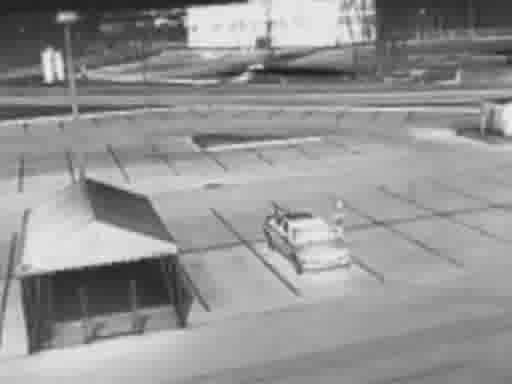
\includegraphics[width=1.2cm]{1.eps}}  %页眉右侧放置logo
\lfoot{}          %页脚左边
\cfoot{\thepage}  %页脚中间
\rfoot{}          %页脚右边
 
 
 
\usepackage{hyperref} %bookmarks
\hypersetup{colorlinks, bookmarks, unicode} %unicode
 

\title{\textbf{\Large{基于颜色分布的内窥镜图像镜面高光检测和修正}}}
\author{ 马佳芮 侯杨清 }
\date{\today}
 

 
\begin{document}
 
\maketitle
%\tableofcontents
 
\begin{abstract}
镜面反射在图像中作为强高亮区域是明显的。这些反射可能成为外科医生的临床观察和判断和基于ar的手术导航的误差的重要来源。本文利用颜色分布,提出了一种以红色通道与绿色和蓝色通道的比率为特征的标准,通过利用红色通道与其他通道之间的差异,并结合重叠窗口,所提出的自适应阈值适用于具有高强度的大高亮区域,这提供了内窥镜图像镜面反射的更可区分的特征。通过对高光区域的精准检测,将高光区域分为不连通的簇,利用高光区域周围的颜色对高光区域进行填充,并利用高斯模糊和掩模衰变最终得到修正图像。经过实验证明,本方案能够精准检测高光区域,并在主观和客观上有较好的恢复效果。
\end{abstract}
 
\begin{center}
\large{\textbf{Abstract}}
Specular reflection is obvious as a strong highlight area in the image. These reflections may become an important source of errors in surgeons' clinical observation and judgment and ar based surgical navigation. This paper proposes a standard characterized by the ratio of red channel to green channel and blue channel by using color distribution. By using the difference between red channel and other channels and combining overlapping windows, the proposed adaptive threshold is applicable to large highlighted areas with high intensity, which provides a more distinguishable feature of mirror reflection of endoscope images. Through the accurate detection of the highlight area, the highlight area is divided into disconnected clusters, the highlight area is filled with the color around the highlight area, and the modified image is finally obtained by using Gaussian blur and mask decay. The experiment proves that this scheme can accurately detect the highlight area, and has a good recovery effect both subjectively and objectively.
\end{center}
 
%\begin{adjustwidth}{1cm}{1cm}
%\hspace{1.5em}Here is the first par. of abstract.Here is the first par. of abstract.Here is the first par. of abstract.Here is the first par. of abstract.Here is the first par. of abstract.Here is the first par. of abstract.Here is the first par. of abstract.Here is the first par. of abstract.Here is the first par. of abstract.Here is the first par. of abstract.Here is the first par. of abstract.
 
%\noindent\hspace{1.5em}Here is the second par. of abstract.Here is the second par. of abstract.Here is the second par. of abstract.Here is the second par. of abstract.Here is the second par. of abstract.Here is the second par. of abstract.Here is the second par. of abstract.Here is the second par. of abstract.
%\end{adjustwidth}
 
\thispagestyle{empty}       %本页不显示页码
\newpage                    %分页
%\tableofcontents\thispagestyle{empty}
\newpage
\setcounter{page}{1}        %从下面开始编页,页脚格式为导言部分设置的格式
 
 
\section{0  引言}
这是第一部分
内窥镜检查是一种诊断程序,它可以让医生观察人体内部。内窥镜通常由连接在细管上的摄像机和光源组成。在内窥镜检查过程中,医生可以在监视器中观察人体内部器官。此外,可以保存带有观察材料的视频,以便进一步分析和处理。由于正面光源,通常镜面反射发生在人体器官表面。镜面反射是当反射角等于入射角时来自表面的光反射的分类。镜面反射在图像中作为强高亮区域是明显的。这些反射是不可取的,因为在许多视觉分析算法中,它们可能成为误差的重要来源。
对于自然图像,大多数方法都是基于各种颜色空间。Xia等人[1]提出了一种通过利用RGB空间中暗通道中的梯度幅度联合色调、饱和度、HSV和RGB空间阈值检测集的方法。基于图像的全局亮度,HSV颜色空间的阈值被自动设置为分离镜面反射[2]。此外,双色反射模型广泛用于自然图像的镜面反射检测[3]。具体而言,该方法使用强度比从图像中提取镜面反射和漫反射分量[4-5]。由于自然图像具有颜色分布和光照不均、高光过度等问题,上述为自然图像设计的方法不适用于内窥镜图像。
对于内窥镜图像,亮点检测方法主要可分为基于不同颜色空间的方法和具有分类器的方法。考虑到内窥镜图像亮点的实时检测,与使用机器学习技术的方法相比,尽管后者可以实现较高的精度,基于颜色空间的方法需要较低的计算[6-7],因此在实践中具有优势。目前,最常用的颜色空间是灰度级[8-9]、HSV[10-11]和RGB[12-13],通过使用不同颜色空间上的预设阈值来确定镜面高光;为了减少高光光环效应的影响,Shen等人[8]提出了一种镜面检测方法,通过采用形态学扩张操作来放大镜面反射区域,该区域通过灰度图像上的预设阈值获得;为了解决镜面反射区域中的某些像素的强度低于非镜面反射区域的问题,Oh等人[10]将镜面反射区域定义为绝对明亮区域和相对明亮区域,这由异常值检测确定。然而,检测到的相对明亮区域可能不仅包括镜面高光,还包括白色组织;Zimmerman Moreno等人[11]使用概率建模从色调和饱和度分量的分割中精确提取高光,以检测粗糙区域内的镜面区域;为了检测强度较低的镜面高光,Arnold等人[13]比较了原始图像和中值滤波图像,通过用周围信息填充每个可能的镜面区域来修改中值滤波图像。除了传统色彩空间的应用,还有一些创新的方法。Akbari等人[14]应用由统计特征训练的非线性SVM分类器,包括从RGB和HSV颜色空间的每个通道提取的平均值和标准差,以评估具有自适应阈值的镜面检测方法;Meslouhi等人[15]应用CIE-XYZ颜色空间的亮度和归一化色度,通过阈值来识别镜面区域。
近年来,高光修正技术可广泛分为两类。一类是基于上述模型的单幅图像去高光方法。Nguyen[16]等人通过分析反射张量的含义和方向信息来评估反射分布,并在高纹理和多色图像上实现良好的突出效果;柴玉婷[17]等人将高光视为噪声,分析漫反射光带和高光光带的光谱,并建立高光滤波器来过滤高光。然而,这些方法受到图像噪声的严重影响,并且它们在不同材料上不具有普适性;Banik[18]等人通过阈值方法用于提取低动态范围图像的高光区域,然后使用邻域像素对其进行修正,然后通过色调映射将修正后的图像转换为高动态范围图像,但这种方法适用于修正具有弱高光的小区域。另一类是基于纹理函数的图像序列。通过分析高光区域周围的纹理函数,匹配并合并从多个角度拍摄的图像,可以保留原始纹理。这一理论于1992年由Lee首次提出,近年来研究者们在修正高光方面取得了一些效果。汪钺杰[19]通过Canny算子提取轮廓函数,匹配左视图和右视图,并在融合后去除塑料膜图像的高光区域。然而,这种方法只能匹配具有旋转误差的图像;何嘉林[20]使用ORB特征点做纹理匹配,通过泊松克隆来恢复高光,但在低纹理的情况下,高光与其他无关区域相比不显著,检测效果不理想;Alsaleh[21]使用基于颜色变化和梯度信息的方法来检测微创手术内窥镜图像中的突出区域,并根据图形数据结构对其进行修正。该方法还需要内窥镜图形的复杂纹理作为分析对象,低纹理图形的修正效果较差。
目前,基于颜色空间的镜面反射检测主要面临两个挑战。一方面,经验阈值是预先设置的,因此不能在不同场景中自适应地调整。另一方面,由于高光和相邻区域之间的有限差异,无法很好地检测高强度的大镜面反射区域[22]。与此同时,现有的大多数高光修正方法大多集中于处理单幅图像或静态场景,一般需要经验阈值设置。然而,这些方法在不同的内窥镜图像序列中很难有效地去除高光。为了解决上述问题,本文在本研究中提出了一种基于内窥镜图像颜色分布特征的自适应检测和修正方法。主要贡献总结如下两点。
(1)利用颜色分布,提出了一种以红色通道与绿色和蓝色通道的比率为特征的标准,通过利用红色通道与其他通道之间的差异,并结合重叠窗口,所提出的自适应阈值适用于具有高强度的大高亮区域,这提供了内窥镜图像镜面反射的更可区分的特征。
(2)通过对高光区域的精准检测,将高光区域分为不连通的簇,利用高光区域周围的颜色对高光区域进行填充,并利用高斯模糊和掩模衰变最终得到修正图像。
 
\section{1  方法描述}
\subsection{1.1  算法描述}
在不失去一般性的情况下,假设高亮像素的强度在周围区域更高,则图像中的该像素定义为:\begin{equation}\label{eq}
  \gamma _2^{\text{C}} = \frac{{{P_{RT}}g}}{{{P_{BT}}d_{_{{B_2}2}}^{ - \alpha } + {N_0}}}
\end{equation} (1)
其中I(x)是像素x 的强度,Imean 是像素x所属的小区域的平均强度,α表示常数参数。计算α*Imean<I(x)的矩阵,并把它放入一个标记矩阵Imeanflag 中,如果α* Imean < I(x) 成立,标记矩阵对应位置置为1,否则为0。上述标准适用于对周围信息更敏感的高强度小镜面区域。然而,由于Imean较高,大镜面反射区域内的像素很难被识别。
为了解决上述问题,本文提出了一种基于RGB颜色空间分布的标准。基本上,在非高光病例中,由于血红蛋白的存在,大多数内窥镜图像呈红色;红色通道的值可能高于绿色和蓝色通道的值。然而,在高光情况下,所有三个通道的值几乎相同且饱和,特别是对于大的高光区域。因此,本文通过使用红色通道与其他通道之间的比率来引入饱和镜面像素的标准:
                                (2)
其中、和分别是像素x的RGB通道的强度。根据(2),非高光像素的R 高于高光像素。因此,引入阈值t来区分高亮和非高亮像素,其定义为:
                               (3)
其中d是每个小区域的红色通道与绿色和蓝色通道之间的差。
                      (4)
其中A表示每个面片中所有像素的集合。利用所定义的阈值,R 低于t 的像素被标记为高光像素。
                                        (5)
然而,对于较暗的像素,所有三个通道的值几乎相同,就像高光像素一样。为了避免黑暗和高光情况之间的混淆,本文需要设置灰度级阈值,先取经验值200。
                                     (6)
使用上述设计的标准,将满足(5)和(6)的图像的像素检测为高亮。
为了进一步提高高亮检测阈值标准的适应性,本文通过将图像分割成重叠的等大小窗口来应用分割预处理。
因此,通过为每个贴片设置自适应阈值,可以解决单个光源引起的照明不均匀的问题。具体而言,在每个补丁中,(1)中的Imean 定义为
                              (7)
此外,如(3)和(4)所示,根据每个补丁的信息计算d,这意味着为每个补丁自适应地设置由d计算的(5)中的t。
在进行修正算法之前,根据红色通道饱和度判别以及自适应阈值生成二值的高光区域蒙版X,其中对应于高光反射的像素具有0值。
得到一个高光区域蒙版X后,将高光区域根据是否连通划分为不同的区域。如图1所示,(a)代表原图像(b)代表当前的高光区域蒙版图像,(c)代表当前图中高光区域被分为46个不连通的高光区域,并被标注不同的颜色。
%插入图片
\begin{figure}[H]   %*表示可跨栏,如果不需要可去掉
\centering
\subfigure[$\sum {{I_C}}  < {I_B}$]{
  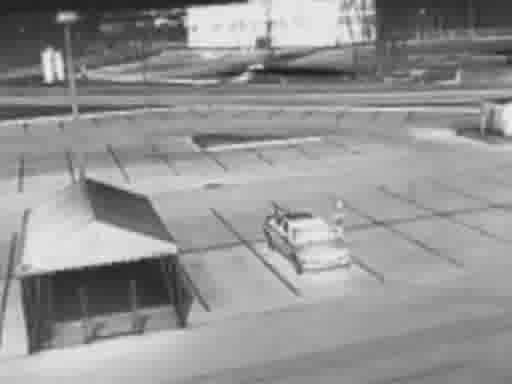
\includegraphics[width=7cm]{1.eps}}
  \hspace{0cm}      %两张图片之间的距离
%\hfill               %撑满整行
\centering
\subfigure[$\sum {{I_C}}  > {I_B}$]{
  \includegraphics[width=7cm]{2.eps}}
\caption{}\label{fig}
\end{figure}

 \subsection{1.2  相关缺陷}
高光区域在数字图像中通常具有一定面积的连通域,高光区域的像素均值较高、方差较小且边缘梯度较大。通常根据上述性质就能检测出高光区域在图像中的位置,但存在的问题是当图像中包含类似上述性质的非高光连通域时,高光区域便难以检测和定位。为剔除无关区,准确检测高光区域,常用显著性识别、阈值处理等方法。采用显著特性提取高光区域容易将原始高光区域过分缩小,造成区域不完整。物体反射率受自身材质、粗糙度、曲率、纹理、光源位置、拍摄角度等因素影响,上文方法所提及的经验阈值200是预先设置的,不能在不同场景中自适应地调整。因此一种需要提供一种灰度级阈值自适应的方法。


\section{2  问题改进}
\subsection{2.1  灰度级阈值设定}
在现有的镜面反射分割方法中,当分析整个图像的直方图并基于高强度像素的峰值分割图像时,阈值技术被广泛使用。图像增强提升反光区域,让反光区域更加明显,让非反光区域更不明显,减少干扰。统计图像的直方图分布,然后对分布曲线做去噪。根据直方图梯度,取最后一个不为零的位置作为阈值thresh。
                                   (8)
\subsection{2.2 方法框架}
在基于颜色分布的内窥镜图像镜面高光检测方法基础上,实现了基于颜色分布的高光修正算法。本文将高光图像划分为连通的不同高光区域。并选取高光区域周围的像素点作为周围区域,寻找周围像素点的最近质心,把质心对应值填充入对应高光区域,得到填充图像利用高斯平滑和掩模衰变对填充颜色进行过度,使得图像更加自然,实现较好的修正效果。如下图呈现的基于颜色分布的内窥镜图像镜面高光检测和修正方法框架图。

\section{3 实验结果与分析}
为证实本文所提到的算法的有效性,本文将从主观与客观两种视角入手,对高光检测和修正的有效性展开分析,并分别与文献[8]、文献[13]和文献[15]的检测算法和文献[4]、文献[13]以及文献[23]的修正算法的处理效果进行了对比。
\subsection{3.1实验环境}
实验环境是Matlab R2021b,实验操作系统是Windows 11,计算机硬件配置为Intel i7-10400F,CPU主频为3.3GHz。实验数据来源自CVC-ClinicDB[24]。根据大量的临床实验,实验中(1)的参数α为2.4,(3)中的参数μ1、μ2和μ3分别被设定为-2.151*10-5,2.031*10-3和1.221。

\subsection{3.2高光检测}
3.2.1主观评价
Shen[8]等人提出了一种基于自适应图像修补和神经网络的内窥镜图像内容感知镜面反射抑制方案,为了自动定位镜面反射区域,采用了具有形态学扩张操作的阈值算法。Meslouhi[15]等人提出了一种基于双色反射模型的方法,利用镜面反射区的颜色特性,通过比较标准化CIE xyY空间的亮度分量y和CIE-XYZ空间的亮度y来实现,反射区域的恢复是通过基于局部信息的多分辨率修复技术来完成的,此外,所提出的方法不需要任何操作阈值。Arnold[13]等人提出一种基于非线性滤波和彩色图像阈值的分割方法,先获取到那些很明显的高光区域,再每个像素与平滑非反光区域颜色像素比较,得到反光区域。
为了评估所提出的算法,通过手动标记来自不同结肠镜检查视频的图像集。由于镜面高光对图像分析算法的负面影响主要是由于沿其轮廓的强梯度,因此使用sobel算子计算梯度大小,并将其叠加在图像上,使手动标签在轮廓上非常精确,将轮廓完全包含在标记的镜面区域中。进一步验证所提出方法的优越性,与文献[8]、文献[13]和文献[15]中的基准镜面检测方法进行了比较,如图4所示。图4中所用的图分别是来自临床数据和CVC临床规范的原始图像。如图所示,可以看出由于扩张操作,Shen DF[8]的方法倾向于检测比实际高亮更大的区域。Arnold[13]中的方法由于应用了局部环境信息而无法检测大的镜面高光区域。Meslouhi[15]中的方法中Y>= y的像素都是反光,容易忽视高光周围的联通区域以及一些小的高光区域。本文方法可以获得准确的高光检测结果,并可以考虑大和小的高光区域。
%插入图片
\begin{figure}[H]   %*表示可跨栏,如果不需要可去掉
\centering
\subfigure[$\sum {{I_C}}  < {I_B}$]{
  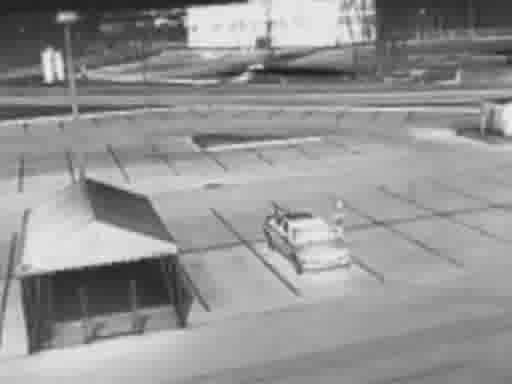
\includegraphics[width=7cm]{1.eps}}
  \hspace{0cm}      %两张图片之间的距离
%\hfill               %撑满整行
\centering
\subfigure[$\sum {{I_C}}  > {I_B}$]{
  \includegraphics[width=7cm]{2.eps}}
\caption{}\label{fig}
\end{figure}%插入图片
\begin{figure}[H]   %*表示可跨栏,如果不需要可去掉
\centering
\subfigure[$\sum {{I_C}}  < {I_B}$]{
  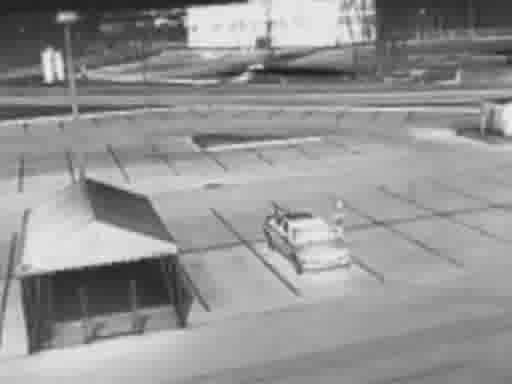
\includegraphics[width=7cm]{1.eps}}
  \hspace{0cm}      %两张图片之间的距离
%\hfill               %撑满整行
\centering
\subfigure[$\sum {{I_C}}  > {I_B}$]{
  \includegraphics[width=7cm]{2.eps}}
\caption{}\label{fig}
\end{figure}

3.2.2客观评价
通过定量评估来评估所提出方法的性能。TPP和FPP分别是在基准和非基准中被检测为高光的像素。类似地,TNP和FNP分别是标记为非高光的像素,它们不在基准范围内。在这项研究中,本文使用精度、准确度来量化所提出的高亮检测方法的性能,其中

\subsection{3.3高光修复}
3.3.1主观评价
主观评价的标准主要是依据人的视觉感受进行判断。下文展示了几种不同方法的修正效果。其中,最左边展示的是原始高光图像,在图像中分布着大小不一的光斑,这些光斑是由内窥镜探头光照造成的镜面高光区域。Shen[4]等人提出了一种方法,在单个像素的基础上实现识别镜面像素。为了处理多色和纹理表面,像素被分类到伪色度空间中的不同簇。根据对应的强度计算每个像素的镜面反射分量。该方法在高光去除精度和计算效率都有不错表现。Fu[23]等人提出了一个方法,通过使用L0范数编码系数稀疏性来恢复那些具有镜面高光的区域的漫反射分量。Arnold[13]等人提出一种基于非线性滤波和彩色图像阈值的分割方法和高效的修补方法,首先,算法用反光检测中的填充,将反光区域进行填充,然后做一个高斯模糊,再然后结合原图和高斯模糊的图进行修复。该算法消除了镜面高光对图像的影响,在视觉上的恢复效果很好。
进一步验证所提出方法的优越性,与文献[4]、文献[23]和文献[13]中的高光修正方法进行了比较,如图5所示。可以看出,前三种方法虽然能够准确地填充高光区域,对其进行修补,但是并没有很好的适应肠道内部的周围环境。Shen[4]和Fu的方法在这个问题上尤其明显,对于局部的点状和片状高光,Shen[4]等人的方法能够较好的定位高光区域,并在小范围的程度上给予灰度填充,但在肉眼观察上恢复效果并不理想;Fu[23]等人的方法的定位区域更加精准范围也更加大,但是主要是起到了掩盖高光区域的效果,并没有对高光区域起到很好的修正效果。Arnold[13]等人的方法可以看出在肉眼上起到了比较不错的修正效果,但是它存在一个问题就是不能够很好的避免内窥镜的边缘对于图像修复过程中产生的影响。在图5的第二行Pic2和第三行Pic3中均有类似边缘模糊现象产生。而本文的方法在很好的视觉效果的基础上,合理的避免了内窥镜图片边缘对修正结果的影响。本文方法在主观视觉上能够修正点状、片状的高光区域,使之颜色与周围区域更好的融合在一起。


3.3.2客观评价
因为高光修正后的图像无论如何都会与原图像产生差别,因此高光图像修正本身并不适合用有参考图像评价指标对高光修正后的内窥镜图像进行评价[25]。本文引入无参考图像质量评估算法NIQE(Natural Image Quality Evaluator),NIQE是一种被用于图像修复领域的评价指标,相较于其他的评价指标。NIQE更符合人眼对图像的主观评价,反映的图像的纹理细节更加符合人眼的视觉习惯,是一种适合图像修复领域的评价指标,NIQE值越大质量越差[26]。
从表中的结果可以看出,本文方法在NIQE指标的表现上普遍较好,与原图对比NIQE指标有明显的下降。此外,与 Fu和Arnold等人的方法比较,也能够有比较不错的表现,能够较大幅度提高图片修正质量。与Shen等人的方法对比,在光线相对充足的图片下,本文方法有着更加好的表现。
%插入表格
\begin{table}[H] \wuhao             %局部字体设置大小
   \centering
  \caption{系统模型符号}\label{tab}
  \begin{tabular}{c|c}
    \toprule                  %设置为顶线默认格式 加粗
    符号 & 说明 \\
    \hline                  %普通横线
    $\alpha$ & 路径衰落系数 \\
    \bottomrule                %设置为底线默认格式
  \end{tabular}
\end{table}
图\ref{fig},式\eqref{eq},表\ref{tab}
最大像素差是反映高光图像是否被有效恢复的一个评价指标,如果高光区域的到有效的修正,则最大像素差应该相较原图有一定的下降。下表是各个高光修正方法的恢复结果。
可见,各个修正方法均能有效的修正高光区域,大幅减少原始图像当中的最大像素差,实现高光区域的修正效果。
%插入表格
\begin{table}[H] \wuhao             %局部字体设置大小
   \centering
  \caption{系统模型符号}\label{tab}
  \begin{tabular}{c|c}
    \toprule                  %设置为顶线默认格式 加粗
    符号 & 说明 \\
    \hline                  %普通横线
    $\alpha$ & 路径衰落系数 \\
    \bottomrule                %设置为底线默认格式
  \end{tabular}
\end{table}
图\ref{fig},式\eqref{eq},表\ref{tab}

像素平均值是反应高光图像在有效修正的同时能否保证与原始图像亮度保持相近的指标。首先,如果图像被有效的修正,像素平均值应该下降,但如果像素平均值出现大幅下降的情况则证明图像的亮度可能存在明显变化。下表展现了各个方法的像素平均值情况(经过归一化处理)。
通过下表,可以清晰的看出本文算法在实现高光图像像素平均值下降的同时,能够较好的保证图像的原始亮度情况。
%插入表格
\begin{table}[H] \wuhao             %局部字体设置大小
   \centering
  \caption{系统模型符号}\label{tab}
  \begin{tabular}{c|c}
    \toprule                  %设置为顶线默认格式 加粗
    符号 & 说明 \\
    \hline                  %普通横线
    $\alpha$ & 路径衰落系数 \\
    \bottomrule                %设置为底线默认格式
  \end{tabular}
\end{table}
图\ref{fig},式\eqref{eq},表\ref{tab}


\section{4  结论}
本文提出了一种用于内窥镜图像的自适应镜面高光检测的方法,主要考虑到内窥镜颜色分布的特点,提出了具有自适应阈值的高光检测标准,并且通过对高光区域的精准检测,将高光区域分为不连通的簇,利用高光区域周围的颜色对高光区域进行填充,并利用高斯模糊和掩模衰变使得图像更加自然,实现较好的修正效果。经过实验证明,本方案能够精准检测高光区域,并在主观和客观上有较好的恢复效果。

 \section{参考文献}
[1]Xia W ,  Chen E ,  Pautler S E , et al. A Global Optimization Method for Specular Highlight Removal from A Single Image[J]. IEEE Access, 2019, PP(99):1-1.
[2]Morgand A ,  Tamaazousti M . Generic and Real-time Detection of Specular Reflections in Images.[C]// 2014 International Conference on Computer Vision Theory and Applications (VISAPP). 0.
[3]Shafer S . Using Color to Separate Reflection Components[J]. Jones and Bartlett Publishers, Inc.  1992.
[4]Hui-Liang, Shen, Zhi-Huan, et al. Real-time highlight removal using intensity ratio[J]. Applied Optics, 2013.
[5]Suo J ,  An D ,  Ji X , et al. Fast and High Quality Highlight Removal from A Single Image[J]. IEEE Transactions on Image Processing, 2016, 25(11):5441-5454.
[6]Sánchez, Francisco Javier,  Bernal J , C Sánchez-Montes, et al. Bright spot regions segmentation and classification for specular highlights detection in colonoscopy videos[J]. Machine Vision and Applications, 2017, 28(8):917-936.
[7]Gao Y ,  Yang J ,  Ma S , et al. Dynamic Searching and Classification for Highlight Removal on Endoscopic Image[J]. Procedia Computer Science, 2017, 107:762-767.
[8]Shen D F ,  Guo J J ,  Lin G S , et al. Content-aware specular reflection suppression based on adaptive image inpainting and neural network for endoscopic images[J]. Computer Methods and Programs in Biomedicine, 2020, 192:105414-.
[9]Chu Y ,  Li H ,  Li X , et al. Endoscopic image feature matching via motion consensus and global bilateral regression[J]. Computer Methods and Programs in Biomedicine, 2020, 190:105370.
[10]Oh J H ,  Hwang S ,  Lee J K , et al. Informative frame classification for endoscopy video[J]. Medical Image Analysis, 2007, 11(2):110-127.
[11]Zimmerman-Moreno G ,  Reinhardt J M ,  Greenspan H , et al. Automatic detection of specular reflections in uterine cervix images[J]. International Society for Optics and Photonics, 2006, 6144:61446E.
[12]Alsaleh S M ,  Aviles-Rivero A I ,  Hahn J K . ReTouchImg: Fusioning From-Local-to-Global Context Detection and Graph Data Structures for Fully-Automatic Specular Reflection Removal for Endoscopic Images[J]. Computerized Medical Imaging and Graphics, 2019.
[13]Arnold M ,  Ghosh A ,  Ameling S , et al. Automatic segmentation and inpainting of specular highlights for endoscopic imaging[J]. Journal on Image and Video Processing, 2010.
[14]Akbari M ,  Mohrekesh M ,  Soroushmehr S , et al. Adaptive specular reflection detection and inpainting in colonoscopy video frames[J]. IEEE, 2018.
[15]Othmane, El, Meslouhi, et al. Automatic detection and inpainting of specular reflections for colposcopic images[J]. Central European Journal of Computer Science, 2011.
[16]Nguyen T ,  Nhat V Q ,  Kim S H , et al. A novel and effective method for specular detection and removal by tensor voting[C]// IEEE International Conference on Image Processing. IEEE, 2015.
[17]柴玉亭, 王昭, 高建民,等. 基于频域滤波的高光去除方法[J]. 激光与光电子学进展, 2013, 50(5):9.
[18]Banik P P ,  Saha R ,  Kim K D . HDR image from single LDR image after removing highlight[C]// 2018 IEEE International Conference on Consumer Electronics (ICCE). IEEE, 2018.
[19]汪铖杰. 基于多视角的去高光技术及应用[D]. 上海交通大学.
[20]何嘉林, 唐露新, 林永强. 基于融合技术的图像去高光方法[J]. 科学技术创新, 2018(6):90-92.
[21]Alsaleh S M ,  Aviles-Rivero A I ,  Hahn J K . ReTouchImg: Fusioning From-Local-to-Global Context Detection and Graph Data Structures for Fully-Automatic Specular Reflection Removal for Endoscopic Images[J]. Computerized Medical Imaging and Graphics, 2019. 
[22]Voronin V ,  Semenishchev E ,  Zelensky A , et al. Specular reflection detection algorithm for endoscopic images[J]. Electronic Imaging, 2019, 2019(11):222-1-222-6.
[23]Fu G ,  Zhang Q ,  Song C , et al. Specular Highlight Removal for Real world Images[J]. Computer Graphics Forum, 2019, 38(7):253-263.
[24]Sánchez, F. J., Bernal, J., Sánchez-Montes, C., de Miguel, C. R., & Fernández-Esparrach, G. (2017). Bright spot regions segmentation and classification for specular highlights detection in colonoscopy videos. Machine Vision and Applications, 28(8), 917-936.
[25]MITTAL A, SOUNDARARAJIAN R, BOVIK A C. Making a “Completely Blind” Image Quality Analyzer[J]. IEEE Signal Processing Letters. 2013,20(3):209-212.
[26]池月,李正平,徐超,冯博.医用内窥镜高光移除算法[J/OL].计算机应用:1-6.

\end{document}